% paper.tex
% sample ACM SIG Proceedings document using LaTeX2e
% Author: Heila van der Merwe
% based upon LaTeX2.09 Guidelines, 9 June 1996
% Revisions:  17 July 2012
%
\documentclass{acm_proc_article-sp}
\begin{document}


\title{Verifying Android Applications using Java PathFinder}

\numberofauthors{3}

\author{%
\alignauthor Heila van der Merwe\\
       \affaddr{Dept. of Computer Science}\\
       \affaddr{University of Stellenbosch}\\
       \affaddr{Private Bag X1 Matieland}\\
       \affaddr{South Africa, 7602}
       \email{hvdmerwe@cs.sun.ac.za}
\alignauthor  Brink van der Merwe\\
 \affaddr{Dept. of Computer Science}\\
       \affaddr{University of Stellenbosch}\\
       \affaddr{Private Bag X1 Matieland}\\
       \affaddr{South Africa, 7602}
       \email{abvdm@cs.sun.ac.za}
\alignauthor  Willem Visser\\
 \affaddr{Dept. of Computer Science}\\
       \affaddr{University of Stellenbosch}\\
       \affaddr{Private Bag X1 Matieland}\\
       \affaddr{South Africa, 7602}
       \email{wvisser@cs.sun.ac.za}
}

\maketitle

\begin{abstract}
Mobile application testing is a specialised and complex field. Due to mobile applications' event driven design and mobile runtime
environment, there currently exist only a small number of tools to verify these applications.

This paper describes the development of JPF-ANDROID, an Android application verification tool. JPF-ANDROID is built on Java PathFinder, 
a Java model checking engine. JPF-ANDROID provides a simplified model of the Android framework on which an Android application can run. It then allows
the user to script input events to drive the application flow. JPF-ANDROID provides a way to detect common property violations such as deadlocks and runtime exceptions
in Android applications. The paper also provides an example of how to apply JPF-ANDROID to an application.
\end{abstract}ii

\category{D.2.5}{Software Engineering}{Testing and Debugging}[Testing tools]

\terms{VERIFICATION}

\keywords{Mobile Application, Java PathFinder, JPF, Android, Verification, Testing}

\section{Introduction}
Software testing and verification plays an important role in determining the quality and robustness of software. These are two very
important attributes of mobile applications. Especially since users currently have more than 600 000 applications to choose from on the
Google Play Market.

Although application testing is so important, it is often neglected due to its complex and time consuming process. Android
applications also face additional challenges when it comes to software testing.

Firstly, they have an event based design which means that their application flow is driven by graphical user interface (GUI) and system
events.

Secondly, Android applications are developed in a custom implementation of the Java Application Programming Interface (API)
 adopted from the Apache Harmony~\cite{harmony} project. The compiled applications can only be executed on a special virtual machine (VM)
called the Dalvik VM that runs on Android devices~\cite{dalvik}.

Due to these challenges, the rapid pace at which applications are developed and the lack of testing tools available, mobile application
testing becomes too expensive in terms of time and money. 

The simplest way to test GUI applications is manual black-box testing, but this is time consuming, error prone
and expensive~\cite{AccessibilityTech}. One way to reduce this high cost, is to 
automate the testing of GUI -- in this case Android -- applications~\cite{AccessibilityTech}.

Currently, Android applications can be tested automatically in one of two ways:

The most common way is to run tests on the Dalvik VM of a physical device/emulator. Testing frameworks such as the MonkeyRunner and
Robotium makes use of Android's built-in JUnit framework~\cite{TestingAndroid} to execute tests on the emulator/device. Other projects use
alternative ways to automatically generate input by manipulating the built in accessibility technologies~\cite{AccessibilityTech} or by
re-implementing the Android keyboard~\cite{KeyboardModel}. Mockito and Android Mock allow JUnit testing on the Dalvik VM by using  mock 
Android classes.

The advantage of testing applications on the Dalvik VM is that Android applications are designed to run on an Android
device and we can physically emulate the input events. The disadvantage is that it is not simple to automate input event emulation. Moreover
running test on the Dalvik VM is slow as they have to be instrumented and each test sequence has to be defined and executed sequentially.

The other approach is to test Android applications by using the Java Virtual Machine (JVM). There are different ways of implementing such
a framework. Android
lint~\cite{lint}, for example, makes use of static analysis to identify common errors in applications. Robolectric~\cite{robolectric}
intercepts the loading of Android classes and then uses shadows classes that model these classes to allow JUnit testing on the JVM.

Although Android applications and Java desktop applications are designed for completely different Java VMs, they are both
built on an implementation of the Java API. As a consequence, Android applications contain many of the
same errors as Java applications. These defects include, but are not limited to, concurrency issues and common runtime exceptions such as
NullPointer Exceptions. It follows that existing Java testing frameworks can be adapted to verify Android applications.

% what are we going to do and why 
This paper describes an extension to Java PathFinder (JPF)~\cite{JPFDocs} that enables the automatic verification of Android applications on
the standard Java JVM. 

The next section will provide an overview of JPF and Android and how JPF can be used to test Android applications. Thereafter
the development of the JPF-ANDROID tool will be discussed, followed by a simple example to show how the tool works.


\section{Design}
\subsection{Java PathFinder}
JPF is an automated, open source, analysis engine for Java applications~\cite{JPFDocs}. It is implemented as an explicit state model checker
that includes mechanisms to model Java classes and native method calls (Model Java Interface - MJI Environment), track byte code execution
and
listen for property violations. Additionally, JPF's design encourages developers to create extensions to the framework. Currently there
exist many
extensions including a symbolic execution extension (JPF-SYMBC)~\cite{JPF-SYMB}, data race
detector (JPF-RACEFINDER) and an abstract window toolkit (AWT) extension (JPF-AWT)~\cite{JPF-AWT}.

The JPF-ANDROID will use JPF's extension mechanisms to:
\begin{enumerate}
\item model the Android application framework so that Android applications can run on the JVM,
\item create an input model to simulate user and system input to drive the application flow.
\end{enumerate}

One of the advantages of extending JPF is that it has been rigorously tested and can successfully detect many common defects in Java applications. As soon as
Android applications can run on JPF-ANDROID, common software errors are automatically detected.

The first step in modelling the Android framework is to understand its architecture.

\subsection{Android}
Android is an open source software stack for devices with an advanced RISC Machine (ARM) architecture  such as smartphones.
It consists of the Android operating system (OS), the application framework and an application development toolkit assisting developers to create
applications for the platform~\cite{AndroidDocs}(see Figure 1~\cite{systemserver}).

The Android OS is built on top of a modified Linux kernel. It provides a layer of abstraction on top of its low level functionality such as process,
memory, user, network and thread management. On top of the Android kernel is a set of native libraries. A custom, optimised
version of the JVM called the Dalvik VM is built on these native libraries.

For security reasons every Android application is run as a separate process in its own Dalvik VM instance~\cite{AndroidSecurity}. Hence, applications can only
communicate with each other and the with the Android framework using Android's Binder inter-process communication (IPC)
mechanism~\cite{Binder}. 

\begin{figure}
\centering
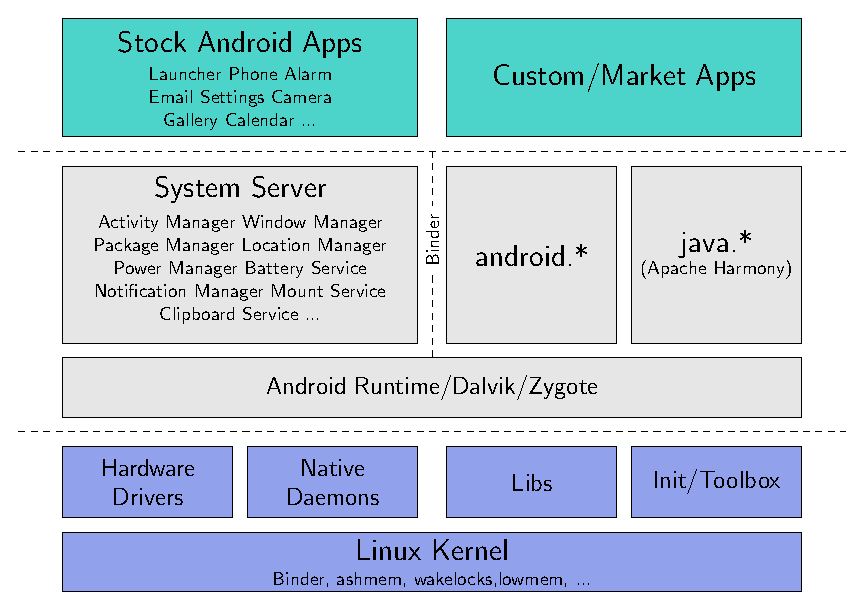
\epsfig{file=Stack.eps, width=3in,}
\caption{The Android application stack}
\end{figure}

The main Android application is called the system process. The system process contains services responsible for running the main tasks of the system for example:
\begin{description}
 \item [ActivityManager] manages the life-cycle and interaction of all the activities running on the system
 \item [WindowManager] allows applications to draw on the screen and forwards UI input to the application.
 \item [PackageManager] stores information on the application packages installed on the device
\end{description}

Android applications follow a single-threaded design in which the main thread of the application handles all application events~\cite{AndroidDocs}. This structure is
commonly used by many UI frameworks since it becomes too complex to make all UI classes thread safe~\cite{SingleThread}. For Android, this main thread is called
the \texttt{Looper}. The \texttt{Looper} has a message queue attached to it containing application events to be dispatched. UI and system
events are scheduled on the main \texttt{Looper} by adding them to the message
queue. The \texttt{Looper} is responsible for continuously looping through these messages and handling them appropriately. This could
include updating a widget, loading a new activity or processing an Intent.

The main class of an Android application is called the \texttt{ActivityThread}. The \texttt{ActivityThread} keeps track of the
application's components and handles user and system events. Android applications consists of the
following application components:
\begin{description}
\item [Activity] responsible for representing and managing an user interface. An application can consist of many
Activities.
\item [Service] performs background operations such as the pulling of messages from a server every 5 minutes. Services do not have user
interfaces and an application can have zero or more services running simultaneously.
\item [Broadcast receiver] listens for and responds to system-wide events such as network failing, low battery or screen orientation
change events.
\item [Content provider] manages application data stored on the file system, in databases, on the web or other storage medium and provides a
gateway to this data from other applications.
\end{description}

These components are created and managed by the \texttt{ActivityManager}. They interact with each other and with other
applications using a structure called an \texttt{Intent}. An \texttt{Intent} is a high level implementation of the Binder IPC.

\subsection{Scope of JPF-ANDROID}
The Android framework is very large and one of the main challenges of JPF-ANDROID is to decide which parts of the system to model. The
objective of JPF-ANDROID is to verify Android applications by executing the code using a collection of different event sequences and then to
detect when certain errors occur.

The more of the Android framework is modelled, the more realistic the model is and the more errors can be found. But, if too much
of the framework is modelled the scheduling possibilities increase exponentially which means that the search space can become too big to
verify.

JPF-ANDROID will focus on verifying one application with multiple application components and their interaction. The system service of the Android OS
is not part of the application process and runs in its own thread. To reduce scheduling possibilities we will not model the entire system
service, but implement the necessary tasks as part of the application process.

The following parts of the Android framework will be modelled:
\begin{description}
 \item [ActivityManager] will manage the life-cycle of Activities and other application components.
 \item [ActivityThread]  will manage the application components and their input.
 \item [Application components] including Activity, Service, Broadcast Receiver and Content Provider. 
 \item [Window and View structure] The view hierarchy will be modelled including the widgets and the window classes.
 \item [Message queue] - The message queue will be modelled to support input from the script file.
\end{description}

Lastly, as the application will not be communicating with outside processes, the \texttt{Intent} objects will be modelled to exclude the
Binder IPC service.

\section{Development}
JPF-AWT introduced the idea of using a simple script file to write event sequences as input to an application. This scripting mechanism makes use of
JPF's state matching and backtracking features to support non-deterministic elements such as the \texttt{ANY} and \texttt{REPEAT}
structures. These structures make it simpler to specify many input sequences simultaneously. As both Android and AWT have a single-threaded
UI design, JPF-ANDROID is built on the design of JPF-AWT. There are two challenges to using this approach:
\begin{enumerate}
 \item Android applications receive input from two different sources: user input and system input where AWT applications only receive user input.
 \item Android applications contain multiple windows - one for each Activity. This complicates the UI input as each
window has its own unique set of view components, hence, a unique input sequence.
\end{enumerate}

\subsection{The JPF-ANDROID input model}
\begin{figure}
\centering
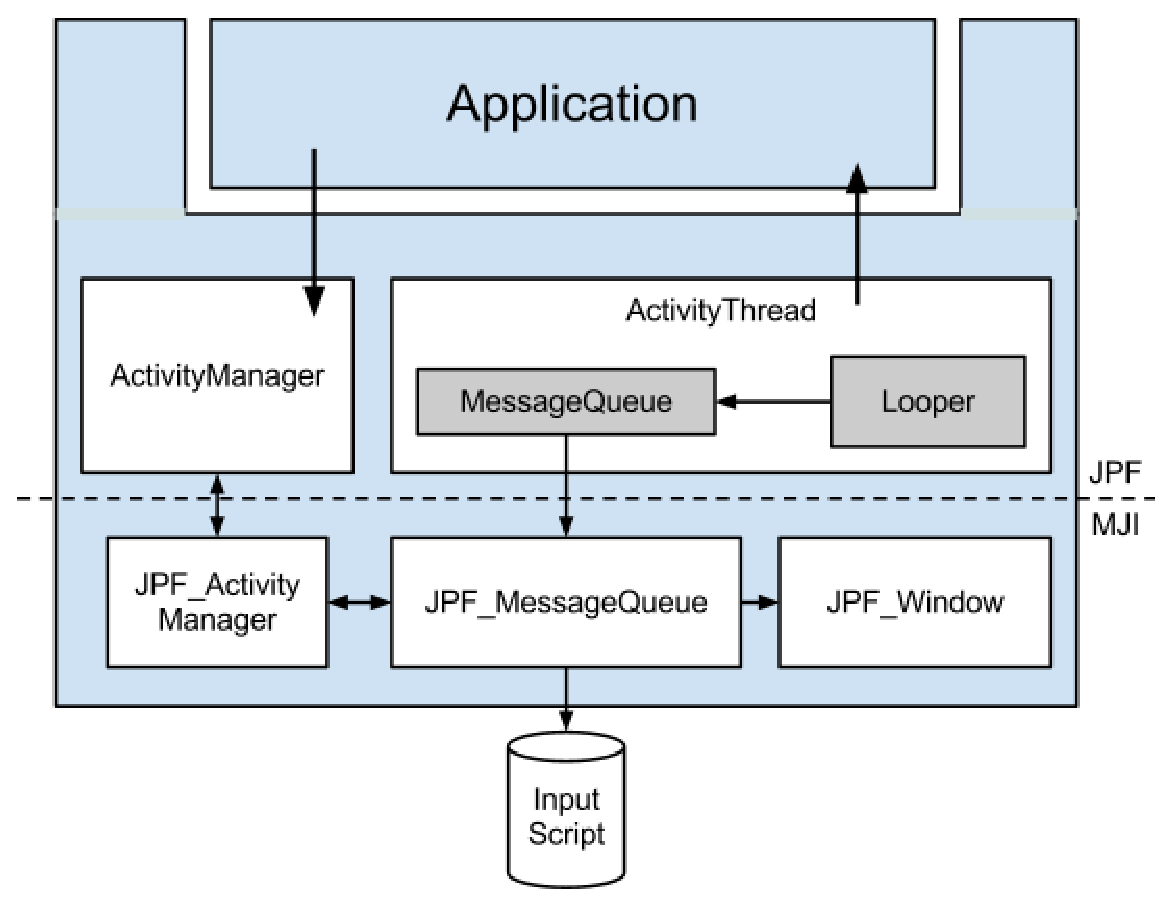
\epsfig{file=arch.eps, width=3.5in,}
\caption{JPF-ANDROID architecture}
\end{figure}

Figure 2 shows JPF-ANDROID's architecture. JPF-ANDROID models Android's message queue structure by using JPF's MJI environment. When the
\texttt{Looper} requests a new message from the 
message queue and it is empty, a call to the native \texttt{JPF\_MessageQueue} class is made. This class reads the next event from the
input script file and classifies it as either a UI event or system event.

UI events are directed to and handled by the native \texttt{JPF\_Window} class. When an Activity's window is inflated, an object map
is created in this native window class. This map binds the name of a widget to the reference of the inflated widget object.
When an UI event is received, the name of the target widget is looked-up in the object map. The action is then called directly on the
inflated widget object by pushing a direct call frame on the JPF call stack. 

System events are a little more complex. They use \texttt{Intent} objects to describe a system event. \texttt{Intents} are used to start
Activities and Services or to provide a notification of certain events. They are similar to messages containing a
description of an operation to be performed or, often in the case of broadcasts, a description of something that has happened and is being
announced~\cite{AndroidDocs}. 

System events are handled by the \texttt{ActivityManager} implemented as the native \texttt{JPF\_ActivityManager} class. The
\texttt{ActivityManager} needs to know which component to send the Intent to: an Activity, Service or Receiver. In an Android
application this information is conveyed by calling one of the following methods: \texttt{startActivity(Intent), startService(Intent),
sendBroadcast(Intent)} from the code. This request is sent to the \texttt{ActivityManager} where it is 
handled appropriately. The  \texttt{ActivityManager} resolves the Intent to the appropriate component and then
schedules the \texttt{Intent} on the application's  message queue. This message will be processed by the \texttt{Looper} which will direct
the event to the \texttt{ActivityThread} to be handled.


To allow a user to script system events, variables were added to the scripting language. Variable names are identified by
the ``@'' in front of the name as '\$' is already used in JPF-AWT to identify UI components. For example a script file that sends an
\texttt{Intent} to start the \texttt{SampleActivity} will contain:

{\small
{\sf
\hspace*{4mm}@intent1.setComponent(``com.example.SampleActivity'')\\
\hspace*{4mm}startActivity(@intent1)\\
\hspace*{4mm}\$button1.onClick()

}
}

\subsection{The input sequence}
JPF-ANDROID started out by using a sequential input script to drive the application execution. This became a problem when some of the
input events were non-deterministically scheduled to happen. In other words, if we do not know whether an event took place or
not, we can not schedule the following events. Lets look at an example:

\begin{figure}
\centering
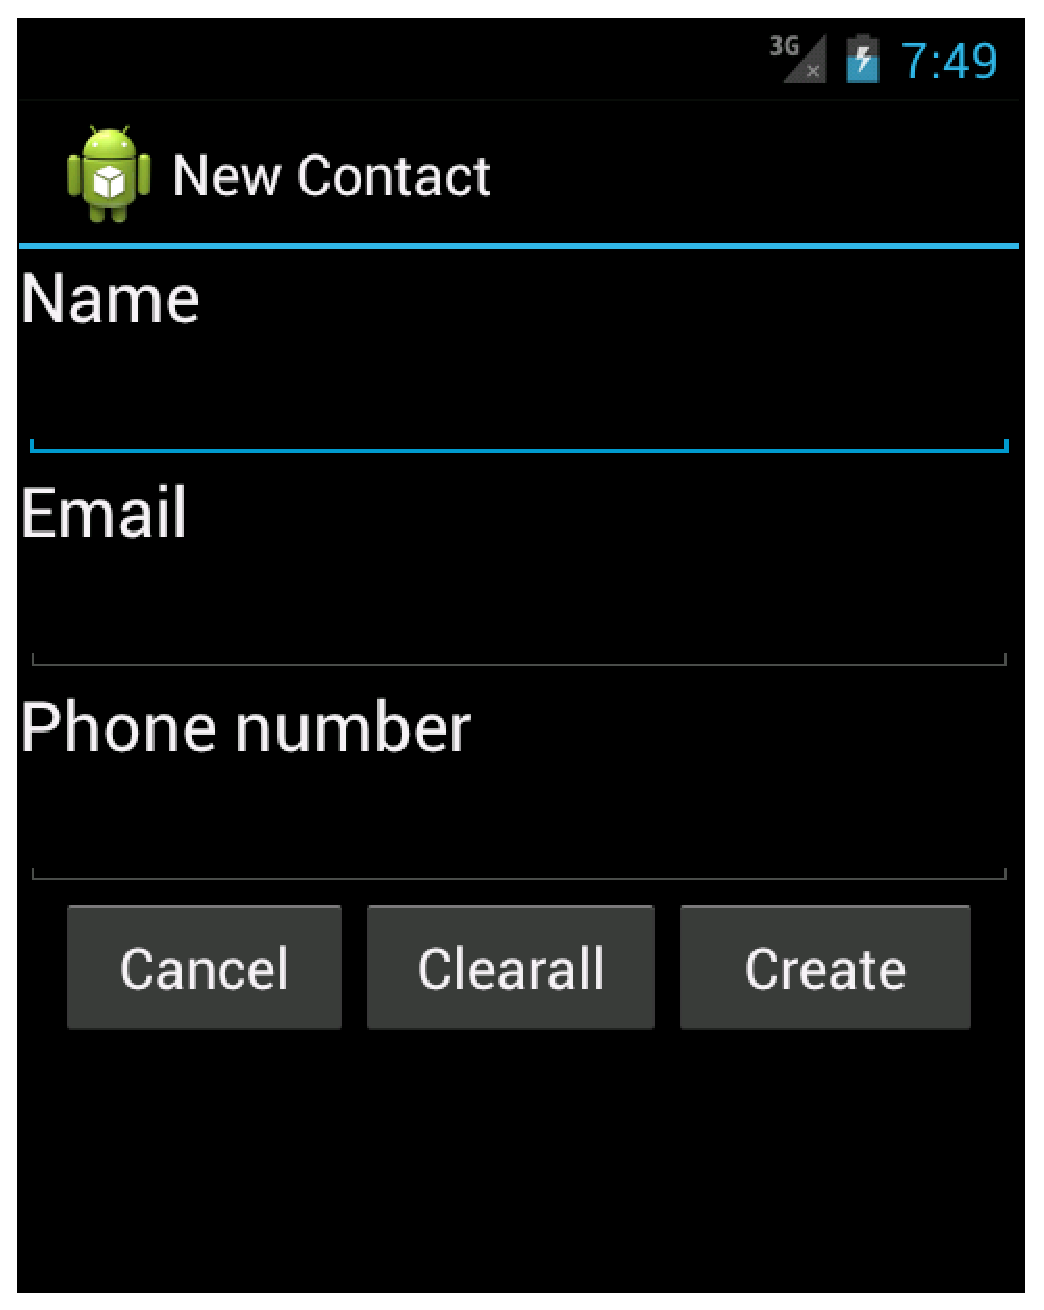
\epsfig{file=newContact.eps, width=1in,}
\caption{Contacts application windows}
\end{figure}

Figure 3 displays the ``Add Contact'' window of a Contacts application. It contains three
buttons: the back button starts the \texttt{ContactsListActivity}, the clear button stays on the current Activity and the create 
button starts the \texttt{ViewContactActivity}. Now let us look at Figure 4 containing the input sequence for the ``Add Contact'' window.

\begin{figure}
{\small
{\sf 
@startIntent.setComponent(``com.example.AddContactActivity'')\\
startActivity(@startIntent)\\
\\
\textbf{REPEAT} 2 \{\\
\hspace*{2mm}\textbf{ANY} \{ \$backButton.onclick(), \$clearButton.onClick()  \}
\}\\
\$nameEdit.setText(``Mary'')\\
\$addButton.onClick() 
}
}
\caption{Non-deterministically starting an Activity}
\end{figure}

This input sequence describes 2 event sequences:
\begin{enumerate}
 \item start AddContactActivity\\
press clearButton\\
set name edit's text\\
press addButton
 \item start AddContactActivity\\
 press backButton button, \\
 set name edit's text\\
 press addButton
\end{enumerate}

The problem is that only after the clear button is pressed is the \texttt{\$nameEdit.setText} command valid. As we do not know
which window is visible after the button press event, we can not use a sequential script. To address this issue, we included the use of
sections in the input script (see figure 5). Each section lists the sequential input of a specific Activity.

\begin{figure}
{\small
{\sf 
\textbf{SECTION} default \{\\
\hspace*{5mm}@startIntent.setComponent(``com.example.ListContactsActivity'')\\
\hspace*{5mm}startActivity(@startIntent)\\
\}

\textbf{SECTION} com.example.ListContactsActivity \{\\
\hspace*{5mm}\$addButton.onClick()\\
\hspace*{5mm}\$list.setSelectedIndex([0-3])\\
\}\\

\textbf{SECTION} com.example.AddContactActivity \{\\
\hspace*{5mm}\textbf{REPEAT} 2 \{\\
\hspace*{7mm}\textbf{ANY} \{ \$backButton.onclick(), \$clearButton.onClick()  \}
\hspace*{5mm}\}\\
\hspace*{5mm}\$nameEdit.setText(``Mary'')\\
\hspace*{5mm}\$addButton.onClick()\\
\}
}
}
\caption{Adding sections to the input script}
\end{figure}

Now, if the back button is pressed the \texttt{ListContactsActivity} will be started and then \texttt{ListContactsActivity}'s event sequence
will execute.

The next challenge is to avoid an infinite loop when returning to an Activity. For example if the back button is pressed on the
\texttt{AddContactActivity} we return to the \texttt{ListContactsActivity}, but, we do not want to repeat the action of pressing on the
addButton again, we want to continue executing the next events. In other words we have to determine when an Activity's event sequence has to
be continued or restarted. We are currently working on this issue.

\section{Case Study}
% example showing the detection of a null pointer exception in certain case
We assume that JPF-CORE and JPF-ANDROID has been downloaded and build in eclipse. To verify an Android application using JPF-ANDROID we
require the source code of the project. In the ``src'' package of the project a script 
file has to be  created including the input events like in figure 6. Also in the ``src'' package has to be a .jpf file that
includes the project setup. Lastly we need to include a stub main method so that JPF-ANDROID has an entry point to the application.

\begin{verbatim}
	/**
	 * The main entry point to the application
	 * 
	 * @param args
	 */
	public static void main(String[] args) {
		  ActivityThread.main(null);
	}
\end{verbatim}

The ViewContactActivity requires an argument containing the contact to view. In this application we did not attach this information to
the starting intent for ViewContactActivity. A null pointer exception occurs when we try to retrieve this value in the ViewContactActivity
and is detected by JPF.

\section{Conclusion}
The paper discussed the design and implementation of JPF-ANDROID. JPF-ANDROID is still under development and currently only models
the core libraries needed to verify a basic Android application. It allows Android applications to be tested using JPF's proven verification
techniques and can successfully detect common Java errors such as runtime exceptions and deadlocks. 

This extension provides a basis on which Android applications can be tested. It can later be extended to verify functional requirements
and identify Android specific errors using JPF's listener mechanism.
\balancecolumns
%
% The following two commands are all you need in the
% initial runs of your .tex file to
% produce the bibliography for the citations in your paper.
\bibliographystyle{abbrv}
\bibliography{paper}  % sigproc.bib is the name of the Bibliography in this case

\end{document}
